\paper{2016}

\question
\begin{parts}
    \part[4]
    Explain what is a compiler and describe the main differences
    between a compiler and an interpreter.

    \part[5]
    Describe when left factoring can be applied to a grammar.
    Illustrate left factoring by an example.

    \part
    \begin{subparts}
        \subpart[3]
        Explain what an ambiguous grammar is.

        \subpart[6]
        Demonstrate with a simple example and using diagrams
        that the following grammar is ambiguous.
        \[
            S \to SaS \mid SbS \mid x
        \]
    \end{subparts}

    \part[7]
    The software tool Lex automatically generates a lexical
    analyser, given a set of patterns (regular expressions)
    with some specific order.
    More specifically, Lex simulates an NFA from the given
    patterns.
    It cans the input string until it finds the longest prefix
    of the input that matches one of the given patterns.
    If this longest prefix matches more than one pattern.
    then Lex chooses among them the pattern that is first in the
    order.

    Let the three patterns in the picture below be given to Lex
    (in this order).
    Assuming that the input string is $xyxx$, find the matching
    pattern of Lex and the longest returned prefix.
    Show all intermediate steps of your computation.
    \begin{center}
        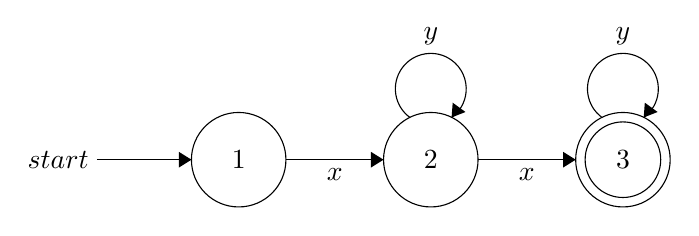
\begin{tikzpicture}[scale=0.2]
            \tikzstyle{every node}+=[inner sep=0pt]
            \draw [black] (14.8,-27.6) circle (3);
            \draw (14.8,-27.6) node {$1$};
            \draw [black] (27,-27.6) circle (3);
            \draw (27,-27.6) node {$2$};
            \draw [black] (39.2,-27.6) circle (3);
            \draw (39.2,-27.6) node {$3$};
            \draw [black] (39.2,-27.6) circle (2.4);
            \draw [black] (5.8,-27.6) -- (11.8,-27.6);
            \draw (5.3,-27.6) node [left] {$start$};
            \fill [black] (11.8,-27.6) -- (11,-27.1) -- (11,-28.1);
            \draw [black] (17.8,-27.6) -- (24,-27.6);
            \fill [black] (24,-27.6) -- (23.2,-27.1) -- (23.2,-28.1);
            \draw (20.9,-28.1) node [below] {$x$};
            \draw [black] (25.677,-24.92) arc (234:-54:2.25);
            \draw (27,-20.35) node [above] {$y$};
            \fill [black] (28.32,-24.92) -- (29.2,-24.57) -- (28.39,-23.98);
            \draw [black] (37.877,-24.92) arc (234:-54:2.25);
            \draw (39.2,-20.35) node [above] {$y$};
            \fill [black] (40.52,-24.92) -- (41.4,-24.57) -- (40.59,-23.98);
            \draw [black] (30,-27.6) -- (36.2,-27.6);
            \fill [black] (36.2,-27.6) -- (35.4,-27.1) -- (35.4,-28.1);
            \draw (33.1,-28.1) node [below] {$x$};
        \end{tikzpicture}
    \end{center}
    \begin{center}
        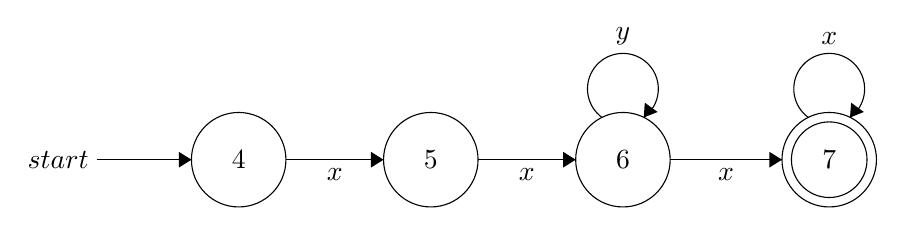
\begin{tikzpicture}[scale=0.2]
            \tikzstyle{every node}+=[inner sep=0pt]
            \draw [black] (14.8,-27.6) circle (3);
            \draw (14.8,-27.6) node {$4$};
            \draw [black] (27,-27.6) circle (3);
            \draw (27,-27.6) node {$5$};
            \draw [black] (39.2,-27.6) circle (3);
            \draw (39.2,-27.6) node {$6$};
            \draw [black] (52.3,-27.6) circle (3);
            \draw (52.3,-27.6) node {$7$};
            \draw [black] (52.3,-27.6) circle (2.4);
            \draw [black] (5.8,-27.6) -- (11.8,-27.6);
            \draw (5.3,-27.6) node [left] {$start$};
            \fill [black] (11.8,-27.6) -- (11,-27.1) -- (11,-28.1);
            \draw [black] (17.8,-27.6) -- (24,-27.6);
            \fill [black] (24,-27.6) -- (23.2,-27.1) -- (23.2,-28.1);
            \draw (20.9,-28.1) node [below] {$x$};
            \draw [black] (37.877,-24.92) arc (234:-54:2.25);
            \draw (39.2,-20.35) node [above] {$y$};
            \fill [black] (40.52,-24.92) -- (41.4,-24.57) -- (40.59,-23.98);
            \draw [black] (30,-27.6) -- (36.2,-27.6);
            \fill [black] (36.2,-27.6) -- (35.4,-27.1) -- (35.4,-28.1);
            \draw (33.1,-28.1) node [below] {$x$};
            \draw [black] (42.2,-27.6) -- (49.3,-27.6);
            \fill [black] (49.3,-27.6) -- (48.5,-27.1) -- (48.5,-28.1);
            \draw (45.75,-28.1) node [below] {$x$};
            \draw [black] (50.977,-24.92) arc (234:-54:2.25);
            \draw (52.3,-20.35) node [above] {$x$};
            \fill [black] (53.62,-24.92) -- (54.5,-24.57) -- (53.69,-23.98);
        \end{tikzpicture}
    \end{center}
    \begin{center}
        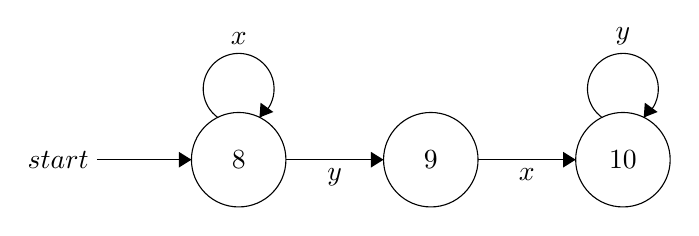
\begin{tikzpicture}[scale=0.2]
            \tikzstyle{every node}+=[inner sep=0pt]
            \draw [black] (14.8,-27.6) circle (3);
            \draw (14.8,-27.6) node {$8$};
            \draw [black] (27,-27.6) circle (3);
            \draw (27,-27.6) node {$9$};
            \draw [black] (39.2,-27.6) circle (3);
            \draw (39.2,-27.6) node {$10$};
            \draw [black] (5.8,-27.6) -- (11.8,-27.6);
            \draw (5.3,-27.6) node [left] {$start$};
            \fill [black] (11.8,-27.6) -- (11,-27.1) -- (11,-28.1);
            \draw [black] (17.8,-27.6) -- (24,-27.6);
            \fill [black] (24,-27.6) -- (23.2,-27.1) -- (23.2,-28.1);
            \draw (20.9,-28.1) node [below] {$y$};
            \draw [black] (37.877,-24.92) arc (234:-54:2.25);
            \draw (39.2,-20.35) node [above] {$y$};
            \fill [black] (40.52,-24.92) -- (41.4,-24.57) -- (40.59,-23.98);
            \draw [black] (30,-27.6) -- (36.2,-27.6);
            \fill [black] (36.2,-27.6) -- (35.4,-27.1) -- (35.4,-28.1);
            \draw (33.1,-28.1) node [below] {$x$};
            \draw [black] (13.477,-24.92) arc (234:-54:2.25);
            \draw (14.8,-20.35) node [above] {$x$};
            \fill [black] (16.12,-24.92) -- (17,-24.57) -- (16.19,-23.98);
        \end{tikzpicture}
    \end{center}
\end{parts}

\question
\begin{parts}
    \part[3]
    Suppose that we have $L$ languages and $M$ machines.
    Assuming that we always build compilers with strict
    separation of the analysis and synthesis phases
    (i.e. front end and back end), how many different modules
    (i.e.front end and back ends) do we need to compile
    all $L$ languages on all $M$ machines?

    \part
    \begin{subparts}
        \subpart[2]
        Describe when a non-terminal in a grammar is called
        left-recursive.

        \subpart[3]
        Eliminate the immediate left recursion in the following 
        grammar.
        \[
            X \to XYb \mid XaZ \mid Yb \mid a
        \]

        \subpart[3]
        In the following grammar, eliminate the left recursion that
        appears in two steps.
        \begin{align*}
            S &\to aB  \mid Ta \\
            T &\to Sba \mid b
        \end{align*}
    \end{subparts}

    \part[6]
    Consider the following Syntax Directed Definition (SDD),
    construct the annotated parse tree for the computation
    $5 * (2 + 4)$.
    \begin{center}
        \begin{tabular}{cll}
            \toprule
            & Production & Semantic rules \\
            \midrule
            1) & $E \to E_1 + T$ & $E.val = E_1.val + T.val$ \\
            2) & $E \to T$ & $E.val = T.val$ \\
            3) & $T \to T_1 * F$ & $T.val  = T_1.val \times F.val$ \\
            4) & $T \to F$ & $T.val = F.val$ \\
            5) & $F \to (E)$ & $F.val = E.val$ \\
            6) & $F \to \text{\textbf{digit}}$ & $F.val = \text{\textbf{digit}}.val$ \\
            \bottomrule
        \end{tabular}
    \end{center}

    \part[8]
    There are two ways in which a lexical analyser distinguishes
    between keywords (i.e. reserved words) and identifiers.
    Briefly describe these two different ways.
\end{parts}
